%% -*- Mode: LATEX -*-

\documentclass[12pt]{../rhitcsse}
\usepackage{multicol}
\usepackage{graphicx}

\ifx\CSSETHREEFIFTYTWO\undefined
\newcommand*{\CSSETHREEFIFTYTWO}{}
\course{CSSE 352}
\coursename{Video Game Development}
\term{Spring}
\acyear{2024-2025}
\instructor{Robert Williamson}
\fi

% Local Variables:
% mode:latex
% End:

 
\title{Lesson 2 Worksheet}

\makeatletter
\renewcommand{\labelenumi}{\bf Question \@arabic\c@enumi}
\makeatother

\begin{document}

\maketitle

\vspace*{0.15in}\hspace{0.25in}Name:\hrulefill\hspace{0.25in}\hspace{0.25in}

\begin{enumerate}
  \item How are the terms \texttt{GameObject}, \texttt{MonoBehaviour}, and \texttt{Transform} related? 
  \vfill

  \item What is a \texttt{component}? How are they different from \texttt{Objects} in OO languages?
  \vfill

  \item How often is the \texttt{Update()} function on a component called? 
  \vfill
  
  \item Why do we use \texttt{Time.deltaTime} when moving our Squares?
  \vfill
  \clearpage
  \centering
  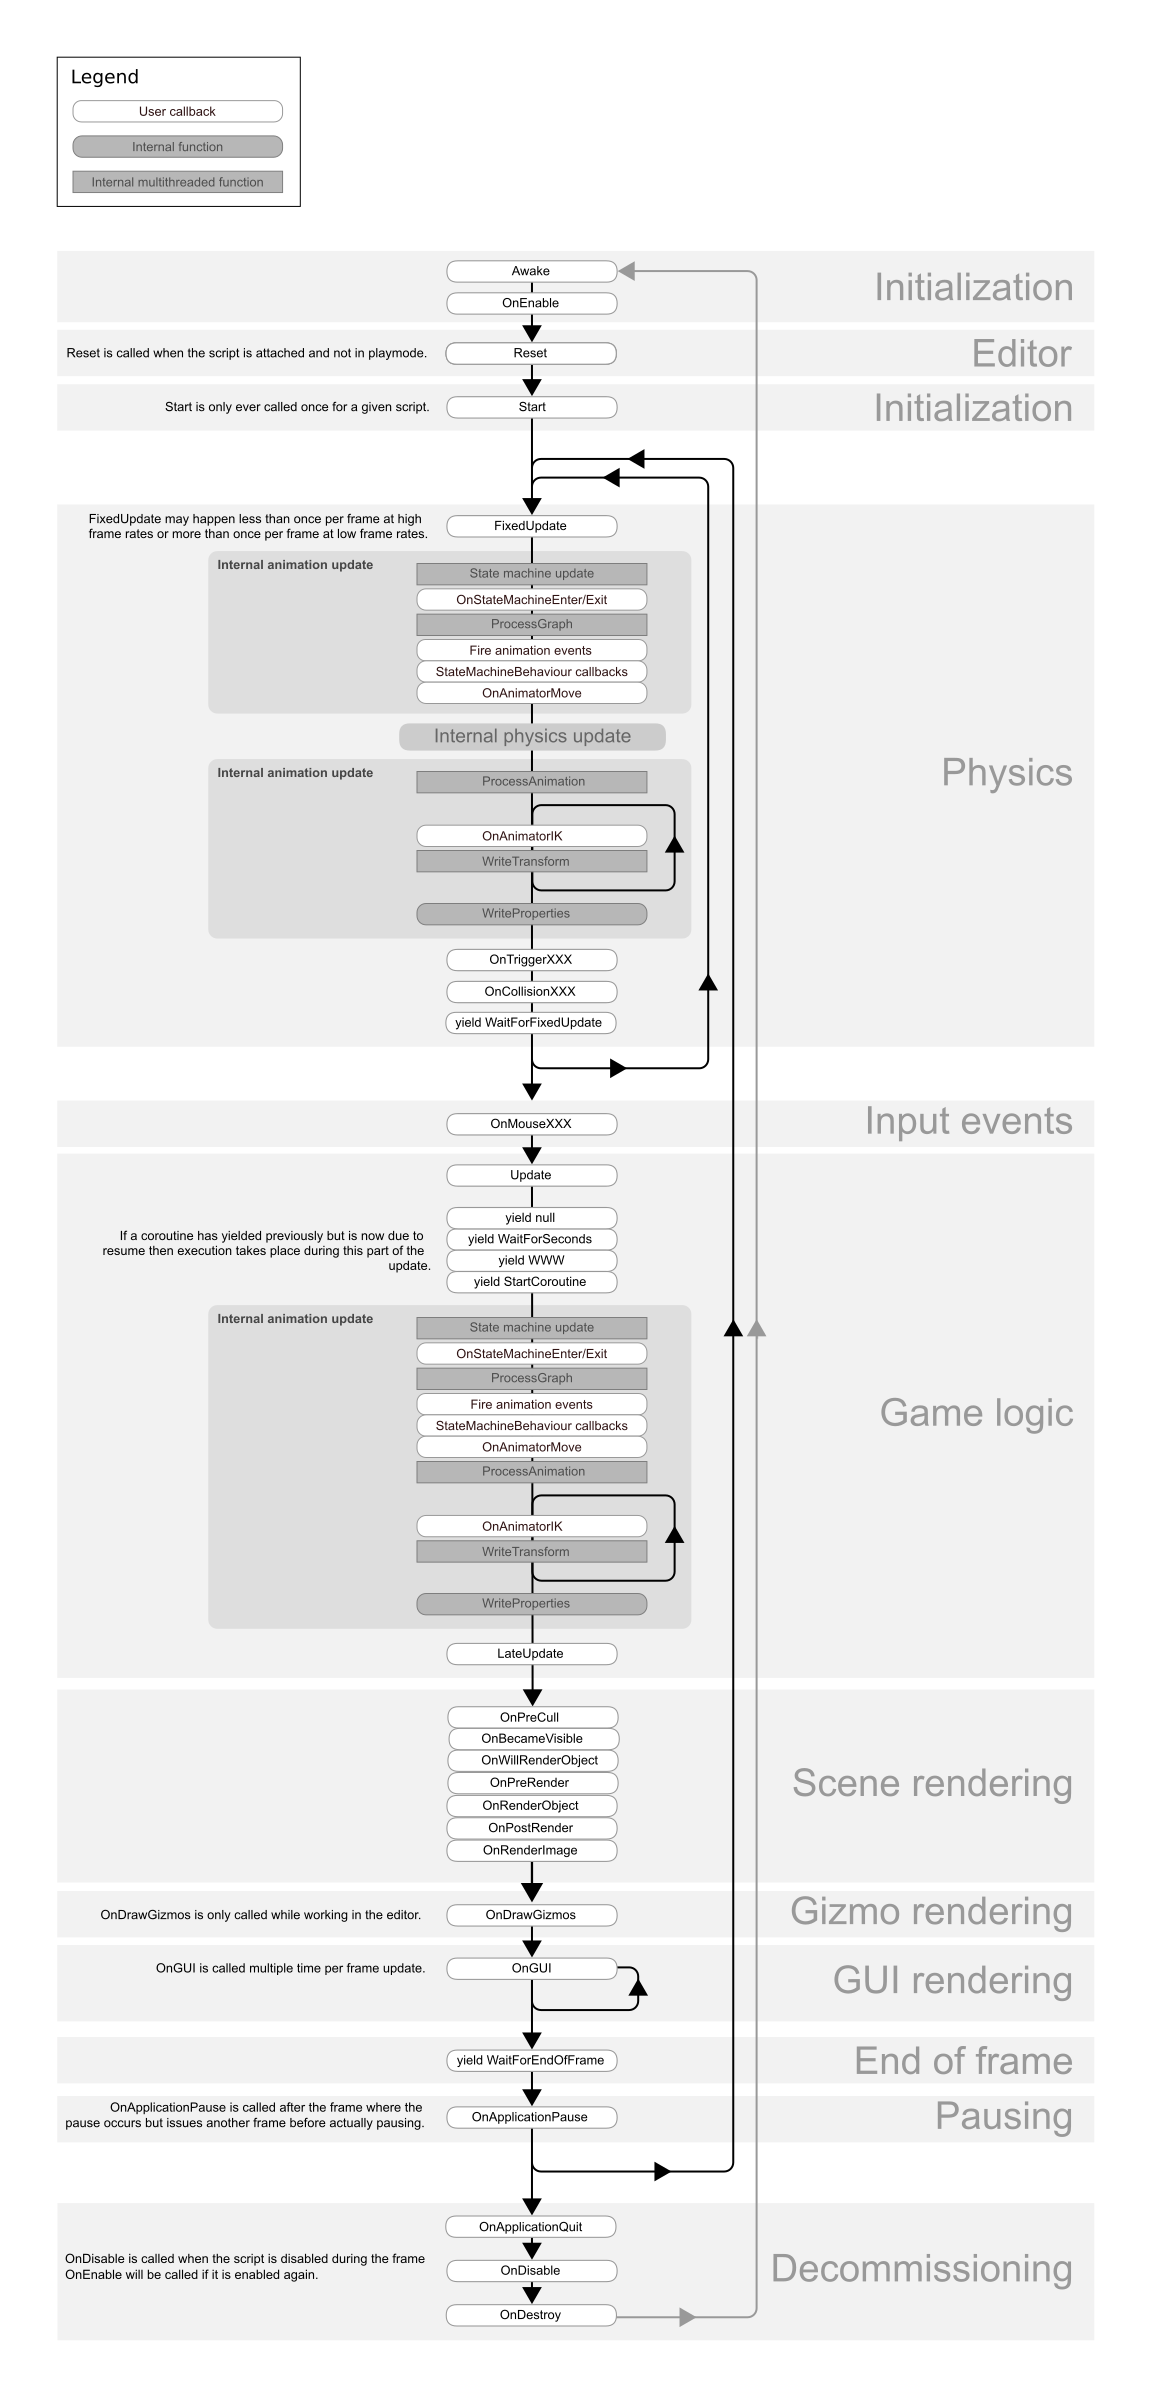
\includegraphics[height=\textheight]{../figs/monobehaviour_flowchart.png}
  
\end{enumerate}

\end{document}

% Local Variables:
% mode:latex
% End:
